\begin{minipage}{1\textwidth}
    In this section, we present the full details of our data analysis.
\end{minipage}
\begin{table}[ht!]
\begin{minipage}{1\textwidth}
\begin{center}
{\small
\begin{tabular}{lrrrrrrrr}
\toprule
& \multicolumn{4}{c}{Training} & \multicolumn{4}{c}{Validation}\\
~ & Max. & Min. & Avg. & Std. & Max. & Min. & Avg. & Std. \\
\midrule
Verb class frequency & 14848 & 73 & 1314 & 2829 & 1937 & 71 & 191 & 398\\
Noun class frequency & 3617 & 178 & 724 & 655 & 430 & 25 & 108 & 92\\
Sentence length & 77 & 3 & 15.1 & 6.3 & 71 & 3 & 14.8 & 6.0\\
Actions per video & 940 & 1 & 136 & 168 & 564 & 3 & 70 & 93\\
Frames per verb class & 2129212 & 20165 & 225170 & 408408 & 407425 & 2702 & 42016 & 76950 \\
Video length & 3708 & 10 & 543 & 645 & 1969 & 11 & 344 & 377 \\
\bottomrule
\end{tabular}}
\caption{Statistics of EPIC-KITCHENS-100 training and validation set}
\label{table:train_val_stats}
\end{center}
\end{minipage}
\end{table}

\begin{figure}[hp]
    \begin{minipage}{1\textwidth}
    \centering
        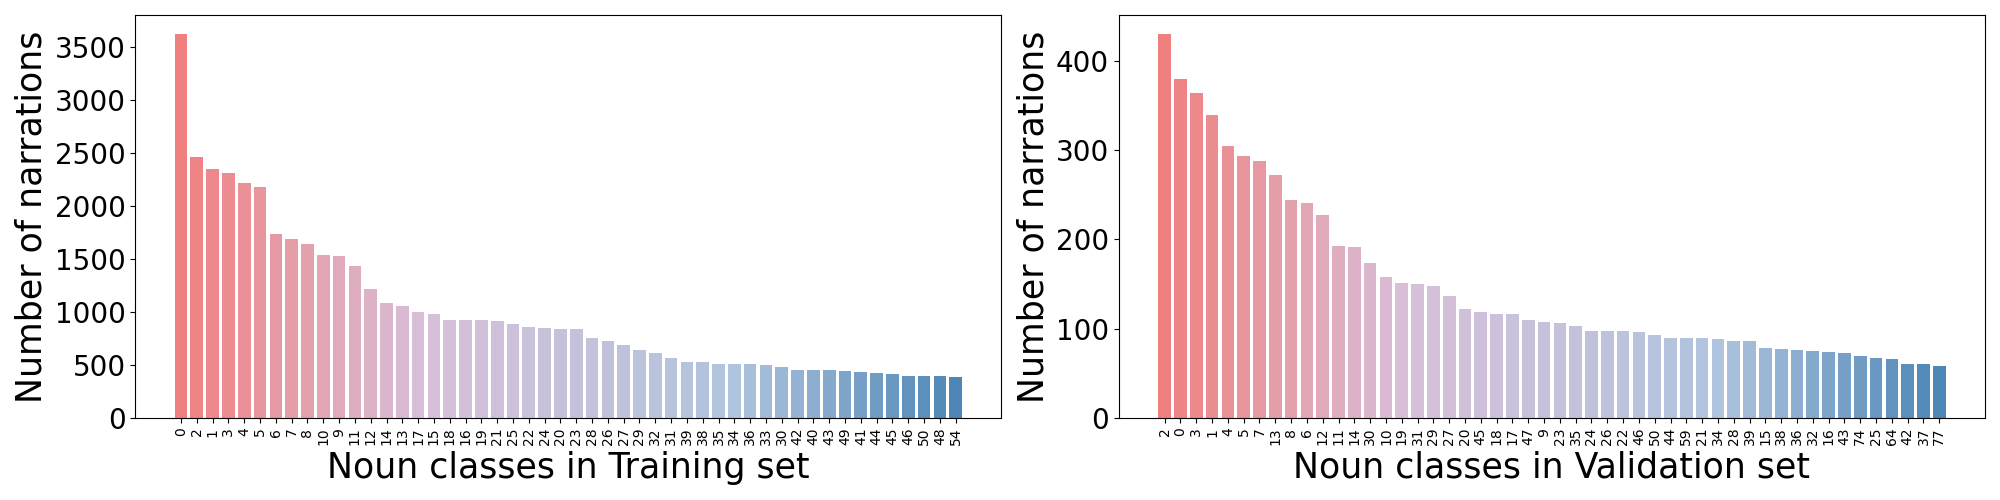
\includegraphics[scale=0.3]{figures/noun_count.png}
    \caption{Frequency distribution of 50 most frequent noun classes in training and validation set}
    \label{fig:noun-freq}
    \end{minipage}
\end{figure}
\begin{figure}[htp!]
    \begin{minipage}{1\textwidth}
        \begin{center}
            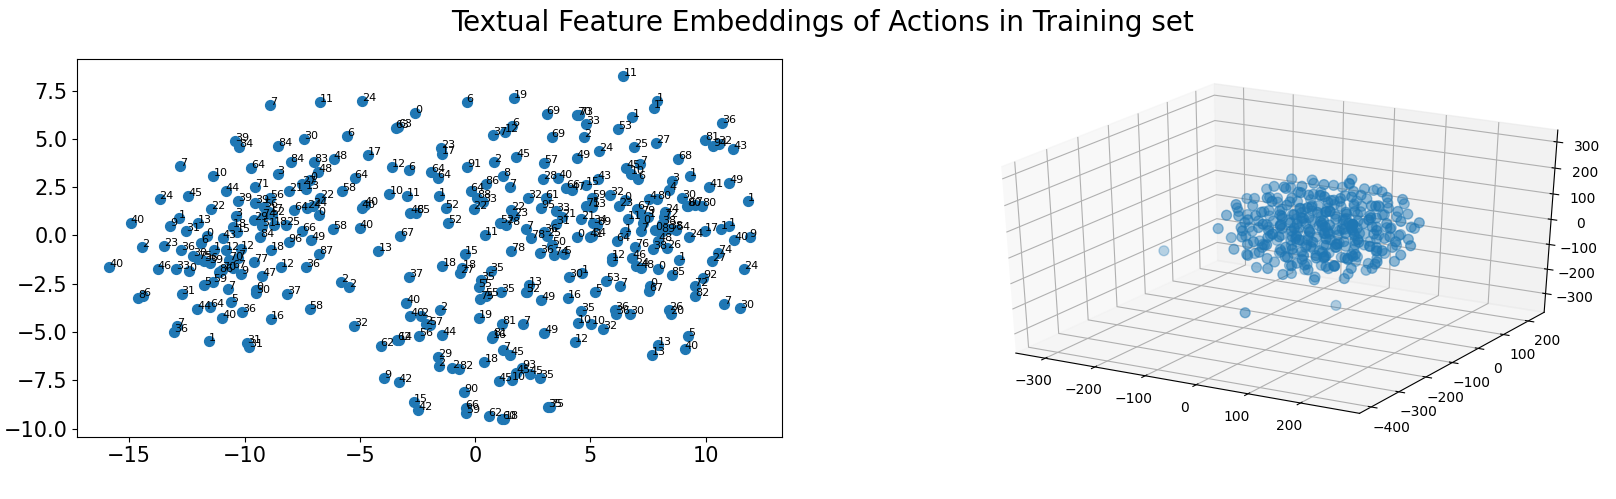
\includegraphics[scale=0.36]{figures/Actions_embeddings_Training.png}
            \\
            \vspace{5mm}
            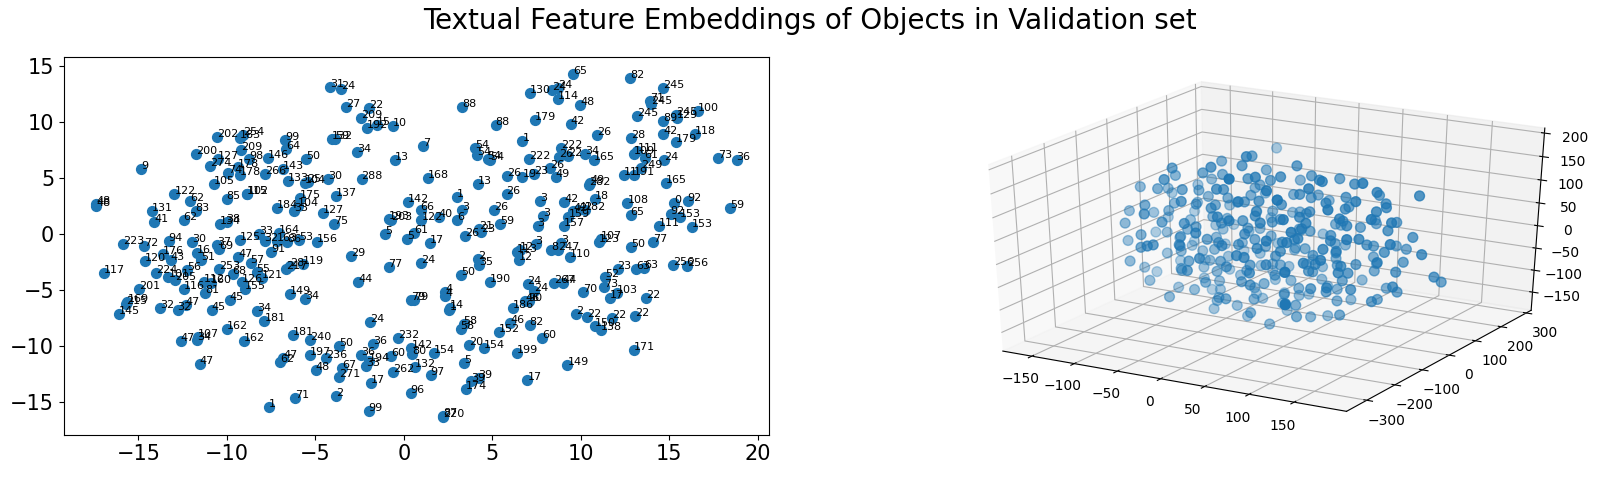
\includegraphics[scale=0.36]{figures/Objects_embeddings_Validation.png}
            \caption{Example of visualizing feature embeddings of verb and noun classes in 2D and 3D space}
            \label{fig:embedding}
        \end{center}
    \end{minipage}
\end{figure}
\clearpage

\begin{figure}[ht!]
    \begin{minipage}[b]{1\textwidth}
        \begin{subfigure}[b]{0.475\textwidth}
            \centering
            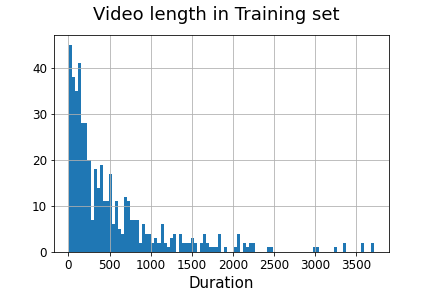
\includegraphics[scale=0.4]{figures/video_length_Training.png}
        \end{subfigure}
        \begin{subfigure}[b]{0.475\textwidth}
            \centering
            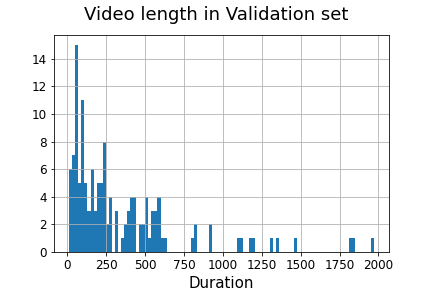
\includegraphics[scale=0.4]{figures/video_length_Validation.png}
        \end{subfigure}
        \caption{Distribution of video length (in seconds)}
        \label{fig:duration}
    \end{minipage}
\end{figure}

\begin{figure}[htp!]
    \begin{minipage}[b]{1\textwidth}
        \centering
        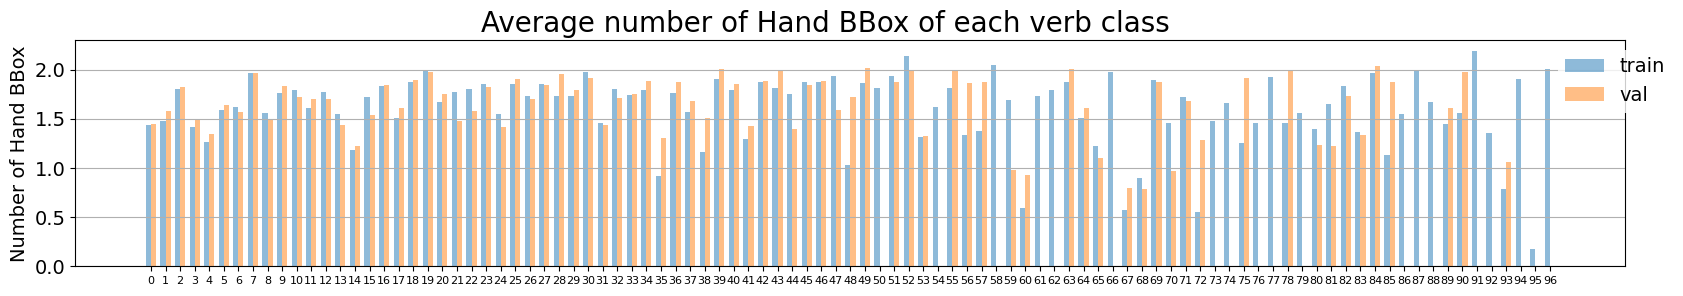
\includegraphics[scale=0.38]{figures/avg_number_Hand_bbox_verb_class.png}
        \caption{Average number of hand bounding-boxes in each frame of given verb class}
        \label{fig:hand-bbox}
    \end{minipage}
\end{figure}

\begin{figure}[htp!]
    \begin{minipage}[b]{1\textwidth}
        \centering
        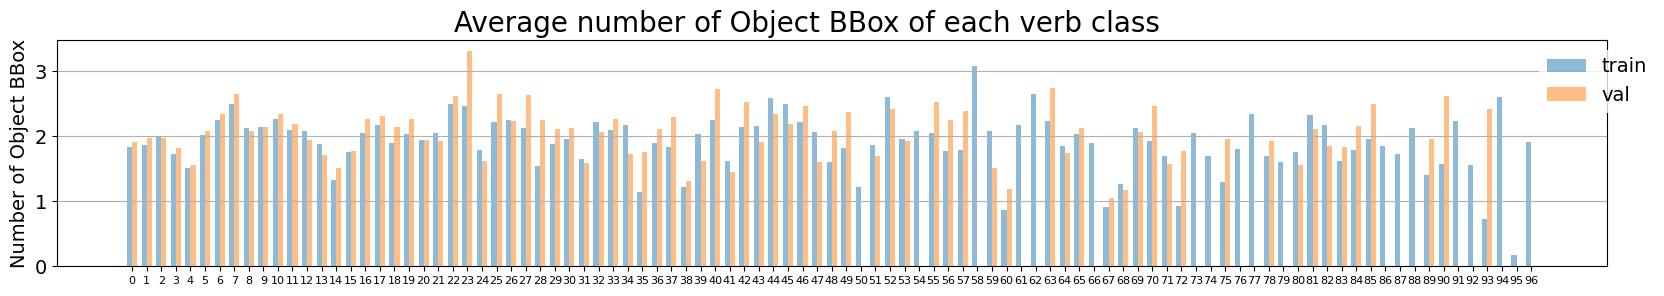
\includegraphics[scale=0.38]{figures/avg_number_Object_bbox_verb_class.png}
        \caption{Average number of object bounding-boxes in each frame of given verb class}
        \label{fig:obj-bbox}
    \end{minipage}
\end{figure}

\begin{figure}[htp!]
    \begin{minipage}[b]{1\textwidth}
        \centering
        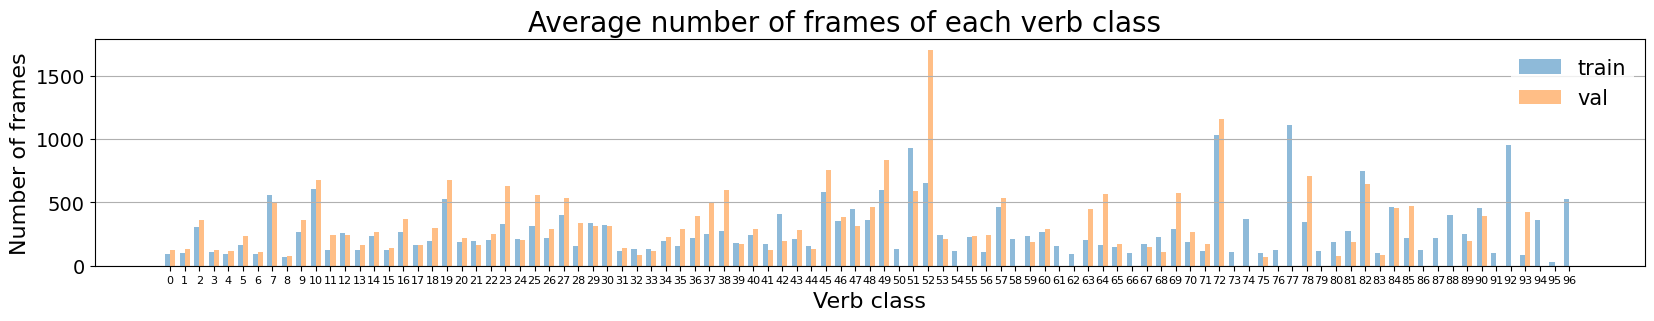
\includegraphics[scale=0.38]{figures/avg_number_frames_verb_class.png}
        \caption{Average number of frames in a narration of a given verb class in training and validation set}
        \label{fig:avg-frame}
    \end{minipage}
\end{figure}

% \begin{figure}[htp!]
% \begin{minipage}[b]{1\textwidth}
%     \begin{minipage}[b]{0.475\textwidth}
%         \begin{subfigure}[b]{0.475\textwidth}
%             \centering
%             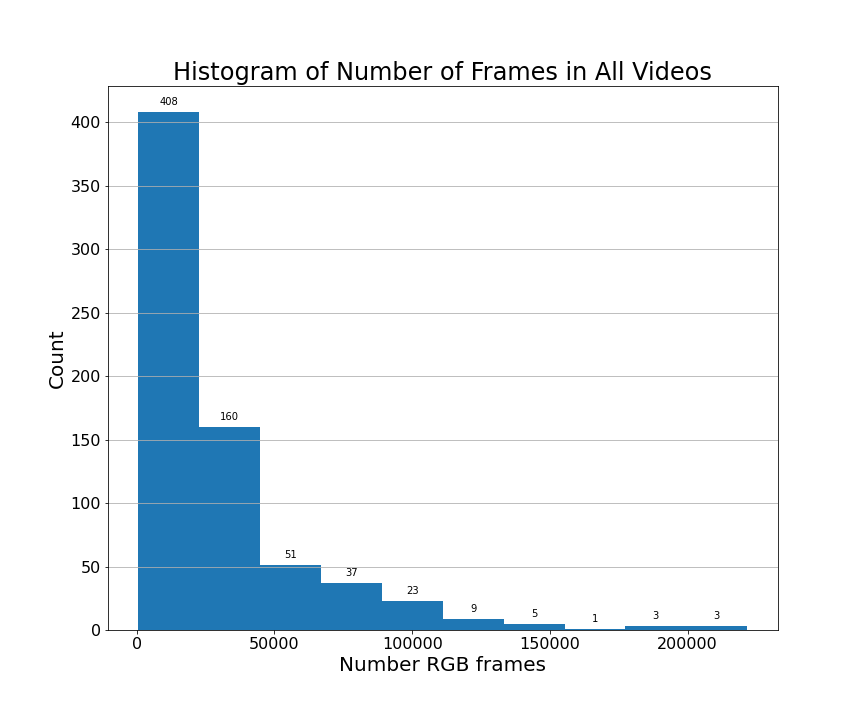
\includegraphics[scale=0.28]{figures/histogram_num_frame_videos.png}
        % \end{subfigure}
        % \begin{subfigure}[b]{0.475\textwidth}
        %     \centering
        %     \includegraphics[scale=0.3]{figures/avg_number_frames_verb_class_4.png}
        % \end{subfigure}
    %     \caption{Distribution of number of frames in each video}
    %     \label{fig:frame-video}
    % \end{minipage}
    % \hfill
    % \begin{minipage}[b]{0.475\textwidth}
    %     \begin{subfigure}[b]{0.475\textwidth}
    %         \centering
    %         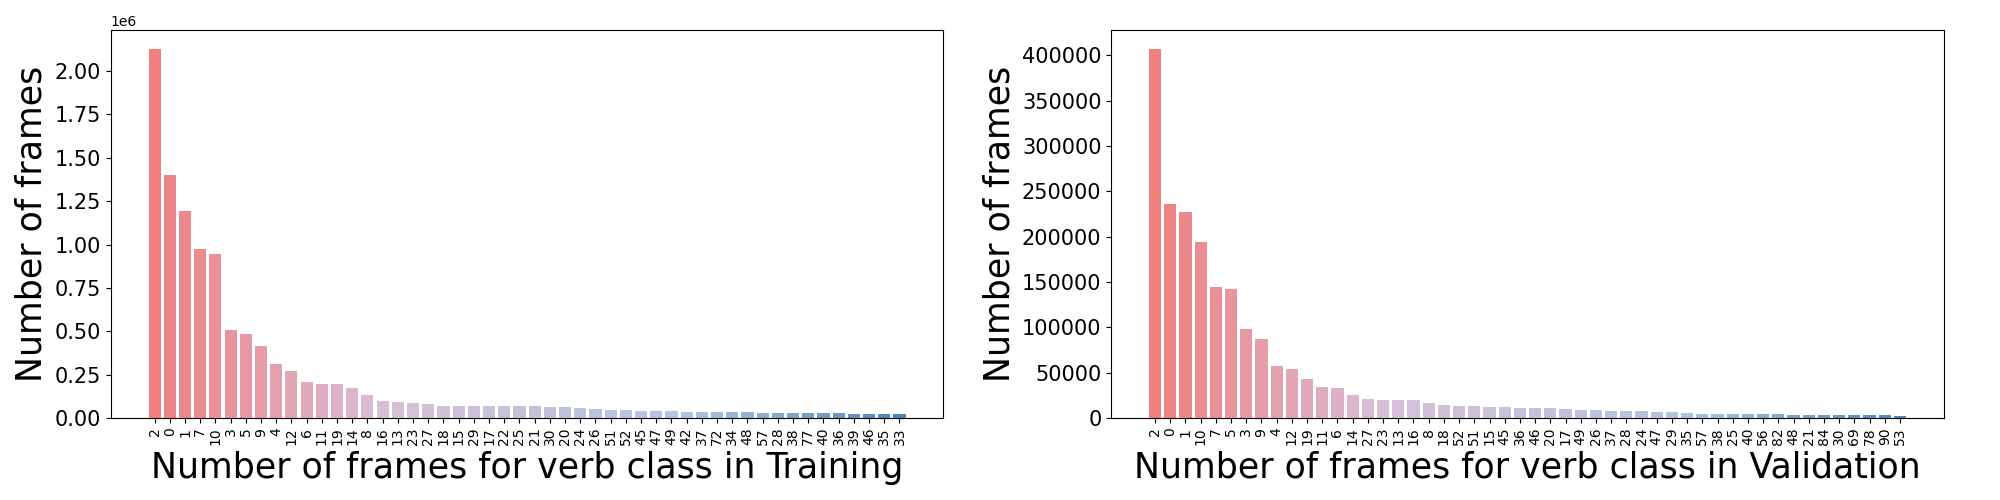
\includegraphics[scale=0.15]{figures/total_frame_word.png}
        % \end{subfigure}
        % \begin{subfigure}[b]{0.475\textwidth}
        %     \centering
        %     \includegraphics[scale=0.3]{figures/avg_number_frames_verb_class_4.png}
        % \end{subfigure}
%         \caption{Distribution of number of frames in each video}
%         \label{fig:total-frame}
%     \end{minipage}
% \end{minipage}
% \end{figure}

% \begin{figure}[htp!]
%     \begin{minipage}[b]{1\textwidth}
%         \begin{subfigure}[b]{0.475\textwidth}
%             \centering
%             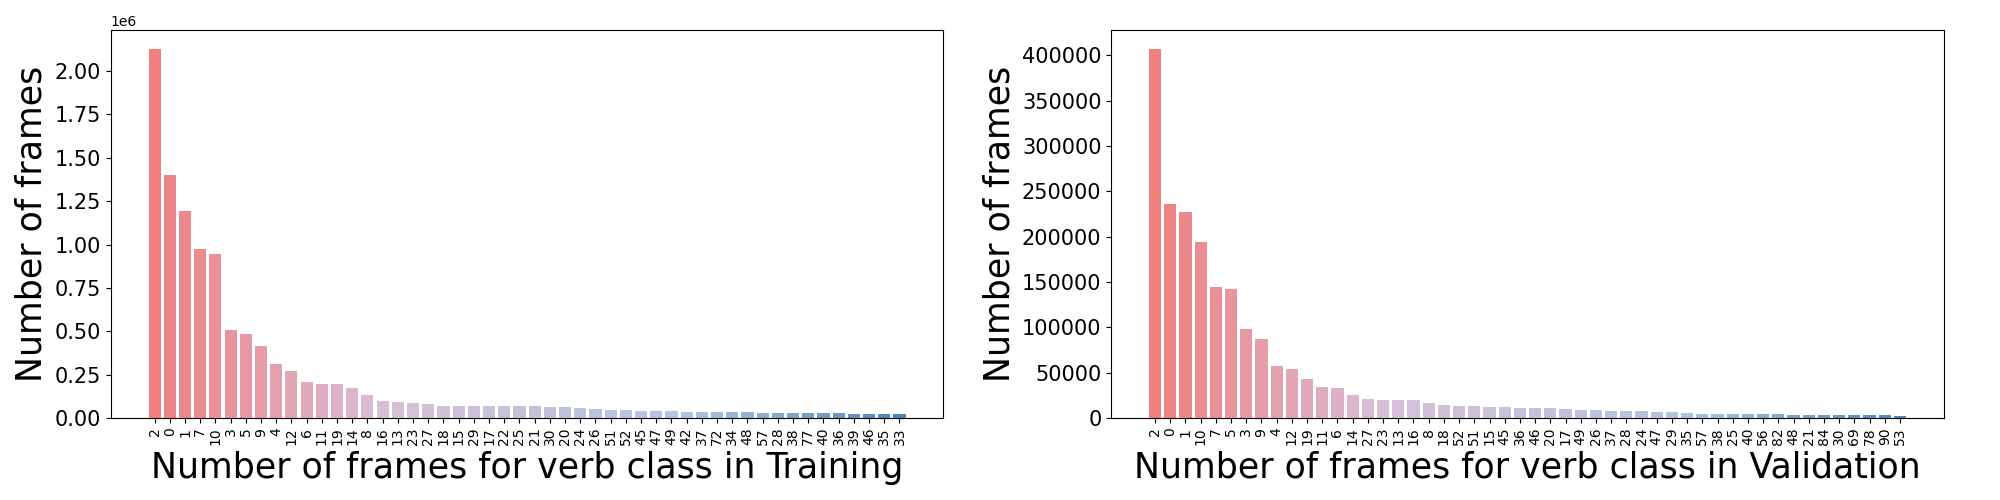
\includegraphics[scale=0.1]{figures/total_frame_word.png}
        % \end{subfigure}
        % \begin{subfigure}[b]{0.475\textwidth}
        %     \centering
        %     \includegraphics[scale=0.3]{figures/avg_number_frames_verb_class_4.png}
        % \end{subfigure}
%         \caption{Histogram of the number of frames in a video}
%         \label{fig:total-frame}
%     \end{minipage}
% \end{figure}

\begin{figure}[htp!]
\begin{minipage}[b]{1\textwidth}
    \centering
    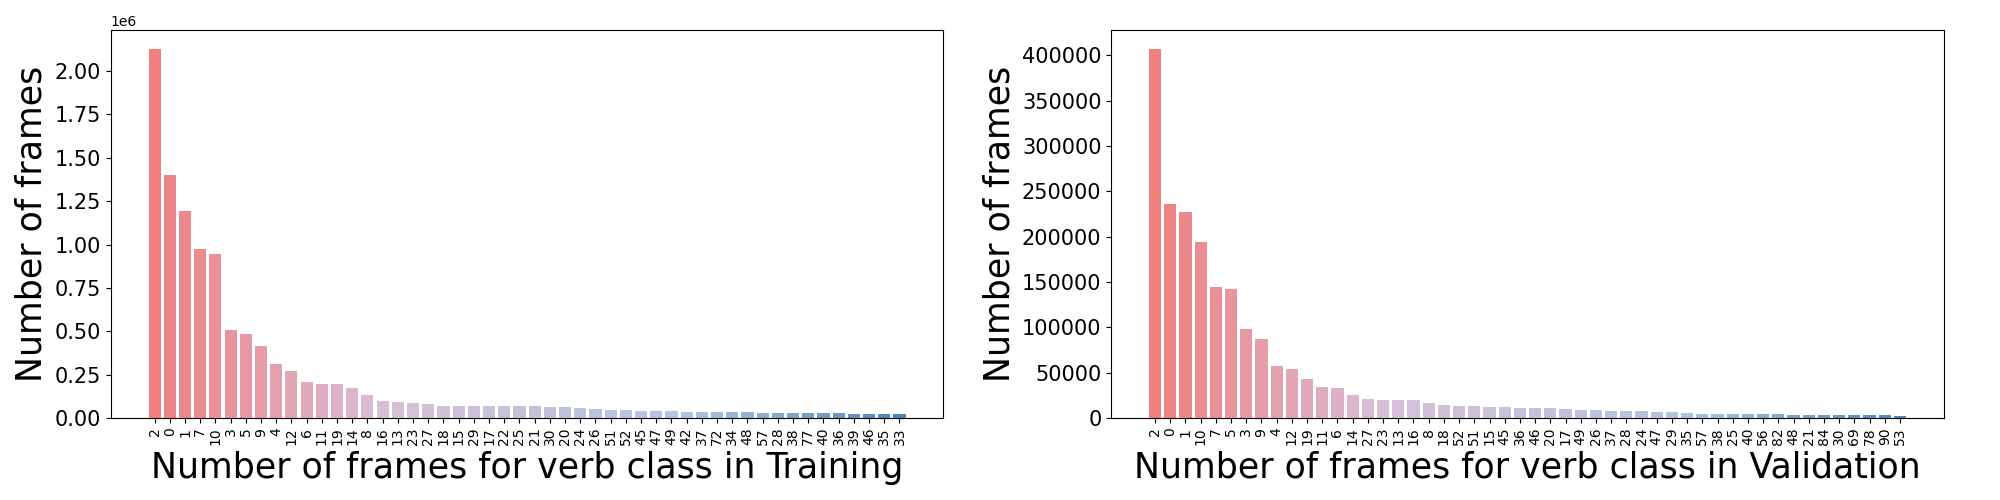
\includegraphics[scale=0.31]{figures/total_frame_word.png}
    \caption{Distribution of number of frames in each video}
    \label{fig:total-frame}
\end{minipage}
\end{figure}

\clearpage

\begin{figure}[t]
    \centering
    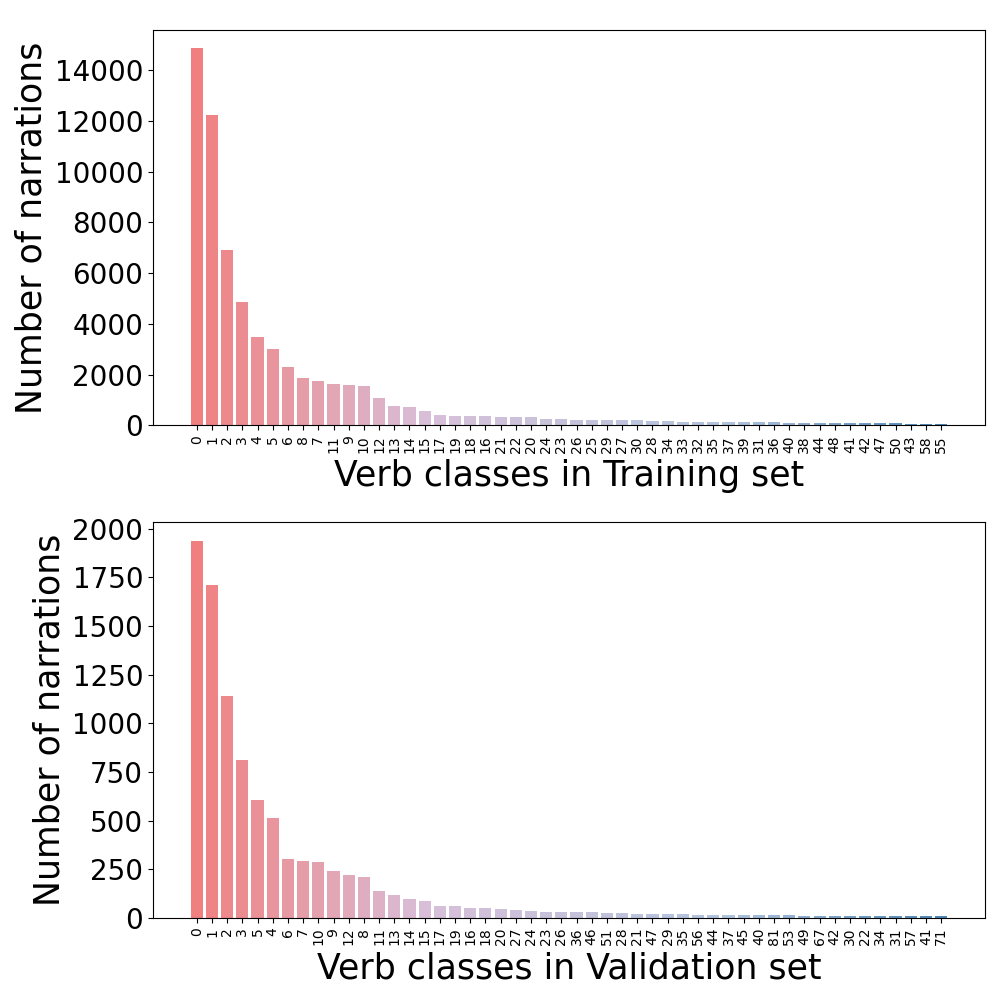
\includegraphics[scale=0.25]{figures/verb_count.png}
    \caption{Frequency distribution of 50 most frequent verb class in training and validation set}
    \label{fig:verb_freq}
\end{figure}

% \subsubsection{Running MSTCN with SlowFast Features} \label{appendix:slowfast}
% We slide 

\begin{figure}[t!]
    % \begin{minipage}[b]{1\textwidth}
        \begin{subfigure}[b]{0.475\textwidth}
            \centering
            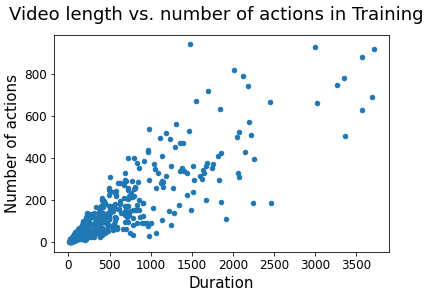
\includegraphics[scale=0.42]{figures/length_vs_actions_Training.png}
        \end{subfigure}\\
        \begin{subfigure}[b]{0.475\textwidth}
            \centering
            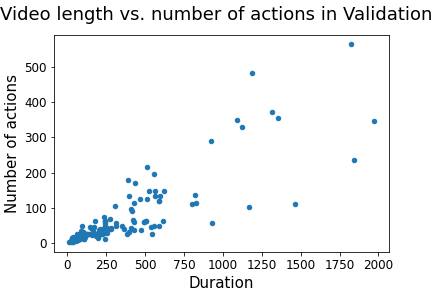
\includegraphics[scale=0.42]{figures/length_vs_actions_Validation.png}
        \end{subfigure}
        \caption{Number of action in each video against video length (in seconds)}
        \label{fig:action-freq-video-length}
    % \end{minipage}
\end{figure}


\subsubsection{Improve Video-Text Matching with Cross-Modal Attention}
The above describes a dual encoder model that independently maps text and video to a joint embedding. It has the advantage in scalability as it can results in efficient evaluation during test time. However, as \newcite{miech2021thinking} points out, it has limited accuracy since the simple dot product is unlikely to capture the complex vision-text interactions. Analogous to how human perform video-text retrieval, one solution is to roughly select a few promising candidates then do fine-grained search for the best candidate by paying more \emph{attention} to visual details. Therefore, we adapt the \emph{Fast} and \emph{Slow} models of \newcite{miech2021thinking} in which the \emph{fast} dual encoder quickly eliminates candidates with low relevance while the \emph{slow} cross-attention model improves retrieval performance with grounding. Given an input segment $\mathbf{v}_i$, we perform retrieval by searching for an action class $\mathbf{c}_j$ such that segment $\mathbf{v}_i$ is most likely to match action class based on the joitnn embedding $\mathbf{c}_j$. Specifically, given segment and action class pair $(\mathbf{v}_i, \mathbf{c}_j)$, we compute their similarity by \[
    h(\mathbf{v}_i, \mathbf{c}_j) = \log (p(\mathbf{c}_j|\phi(\mathbf{v}_i);\theta))
\]
where $\phi(\mathbf{v}_i)$ is extracted feature of segment $\mathbf{v}_i$ and $\theta$ is the parameters of the transformer model. To combine results from dual encoder model and cross-attention model, given input segment $\mathbf{v}_i$ and action class set $\mathcal{C}$ containing $K$ action classes. we first obtain a subset of $m$ action classes $\mathcal{C}_m$ (where $m \ll K$) that have the highest score according to the fast dual encoder model. We then retrieve the final top ranked action class by re-ranking the candidates using the cross attention model:
\[
    \mathbf{y}^*_i=\text{argmax}_{\mathbf{c}_j\in \mathcal{C}_m} h(\mathbf{v}_i, \mathbf{c}_j) + \beta s(\mathbf{v}_i,\mathbf{c}_j)
\]
where $\beta$ is a positive hyper-parameter that weights the output scores of the two models. We output $(\hat{\mathbf{y}}^*_{i,c})$ as the classification probability of frame $i$ as action $c$ based on the similarity score and $(\mathbf{y}^*_i)_{i\in s_i^{3D}}$ as new labels for segment $i,i\in[t]$.
